\subsection{Estudio técnico}
\subsection{Tamaño}
Basandose en el enfoque principal del proyecto, siendo este los nomadas digitales en Bogotá, realizando un análisis del mercado y los recursos necesarios para su desarrollo.El crecimiento del proyecto se verá fundamentado en:

\begin{itemize}
    \item \textbf{Estructura operativa agil:}El proyecto se conformará con un equipo de desarrollo, equipo de analisis de datos y un equipo de marketing, que tendrán un crecimiento escalable y sostenible a lo largo del tiempo.Dichos equipos estarán enfocados en la creación de un producto que se adapte a las necesidades del mercado, permitiendo una rápida adaptación a los cambios y tendencias del sector.
    \item \textbf{Oportunidad de mercado:} Hay un constante crecimiento en el recibimiento de nomadas digitales en Bogotá,pero un gran porcentaje de estos reportan la inseguridad como una barrera para su permanencia en la ciudad,destacando de esta manera la necesidad de un servicio que les brinde seguridad y bienestar,grantizando una mejor experiencia en su estancia.
    \item \textbf{Arquitectura tecnologica:} Plataforma desarrollada con herramientas escalables (AWS, IA para análisis de riesgo) y bajo costo operativo, facilitando el crecimiento proyectado sin sacrificar la calidad del servicio ni aumentar la inversion inicial de manera significativa. La plataforma se diseñará para ser flexible y adaptable, asegurando la integración de nuevas funcionalidades y servicios conforme el mercado evolucione.
\end{itemize}

Comprendiendo estos aspectos, se fundamenta la viabilidad del proyecto, además de su crecimiento y desarrollo sostenido. Supliendo las necesidades del mercado de nómadas digitales en Bogotá, que desean una experiencia segura y de calidad durante su estancia en la ciudad.

\subsection*{Localización}
La localización del proyecto es fundamental para garantizar la conexion con el mercado objetivo y la infraestructura necesaria para su desarrollo. En este caso, se considera la ciudad de Bogotá como el lugar ideal para establecer la sede del proyecto, debido a su creciente comunidad de nómadas digitales y la infraestructura tecnológica disponible.
Para tomar esta decisión, se han evaluado diversos factores:
\begin{itemize}
    \item \textbf{Acceso a talento:} Bogotá cuenta con una amplia oferta de profesionales en tecnología, marketing y desarrollo de negocios, lo que facilita la formación de un equipo competente y especializado.
    \item \textbf{Infraestructura tecnológica:} La ciudad dispone de una infraestructura tecnológica avanzada, con acceso a internet de alta velocidad y servicios de soporte técnico, lo que es esencial para el desarrollo y operación del proyecto.
    \item \textbf{Ecosistema emprendedor:} Bogotá alberga un ecosistema emprendedor en crecimiento, con espacios de coworking, incubadoras y aceleradoras que pueden apoyar el desarrollo del proyecto.
\end{itemize}

\textbf{lugares candidatos:} Considerando los factores mencionados,se han identificado varios lugares en Bogotá que cumplen con los requisitos necesarios para establecer la sede del proyecto. Dichos lugares demuestran tener la infraestructura adecuada, espacios de trabajo colaborativo y acceso a servicios tecnológicos, lo que los convierte en opciones viables para la localización del proyecto.

\begin{itemize}
    \item \textbf{ParqueSoft:} Parquesoft Bogotá es un proveedor multi-sectorial de servicios de Tecnologías de la Información, que funciona con el apoyo de más 50 empresas de base tecnológica en Bogotá, que trabajando juntas generan una oferta de valor integral, creando soluciones de calidad, a la vanguardia con últimas tendencias digitales.Se debe destacar que Parquesoft apoya a empresas emergentes garantizando innovación,pasión y sinergia entre las empresas que allí se encuentran, además de contar con un equipo de profesionales altamente capacitados y comprometidos con el desarrollo tecnológico del país.

\begin{adjustbox}{center, caption={Precios de Espacios en ParqueSoft}, label={ParqueSoftPrecios}, nofloat=table, vspace={20px}}
    \begin{threeparttable}
        \centering
        \begin{tabular}{|p{7cm}|p{8cm}|}  % Definir las columnas de tamaño adecuado
            \hline
            \cellcolor[HTML]{D9EAD3}\textbf{Tipo de Servicio} & \cellcolor[HTML]{D9EAD3}\textbf{Costo Mensual} \\ \hline
            Suscripción Mensual   & \$96.000 - Total Anual: \$1.152.000 \\ \hline
            Suscripción Semestral & \$78.000/Mes - Total Anual: \$932.000 \\ \hline
            Suscripción Anual     & \$69.000/Mes - Total Anual: \$828.000 \\ \hline
        \end{tabular}
        \begin{tablenotes}[para,flushleft]
            \vspace{2mm}
            \textit{Nota. Fuente: ParqueSoft.com}
        \end{tablenotes}
    \end{threeparttable}
\end{adjustbox}

\item \textbf{Decisión:} Realizando una evaluación de las opciones disponibles,Parquesoft demuestra ser el lugar ideal para desarrollar y establecer la sede del proyecto,considerando los precios de los espacios, el enfoque de tecnologia y el apoyo al emprendimiento emergente. Parquesoft ofrece un apoyo integral a las empresas emergentes, permitiendo el correcto desarrollo del proyecto y su posicionamiento en el mercado,manteniendo las bases de innovación,pasión y sinergia.
\end{itemize}

\subsection*{Tipo de emprendiemiento} El proyecto de calatalogará como un Startup,desarrollada bajo la metodologia Lean Startup, ya que esta metodologia se adapta perfectamente a las características del proyecto, permitiendo un enfoque ágil y flexible en el desarrollo del producto. 

La metodología Lean Startup se centra en la creación de un producto mínimo viable (PMV) que permita validar las hipótesis del negocio con una inversión mínima, facilitando la adaptación y evolución del proyecto conforme a las necesidades del mercado.
Esta metodologia permite un enfoque iterativo, donde se construye, mide y aprende de manera continua, lo que es esencial para el desarrollo de un producto innovador y escalable como el propuesto en este proyecto.

La razón de esta metodología es aprender en poco tiempo, invirtiendo los mínimos recursos. Lean Startup es una metodología dirigido a la puesta en marcha de ideas innovadoras, donde no se comienza creando una empresa, sino una Startup, entendida no como una empresa en pequeño, sino como «una institución humana diseñada para crear un nuevo producto o servicio bajo condiciones de incertidumbre extrema» 
\cite{MetodologiaLean}

\begin{minipage}{0.9\textwidth}
        \centering
        \captionof{figure}[{Metodología Lean Startup}]{Ciclo de Desarrollo Lean Startup}
        \label{leanStartUp}
         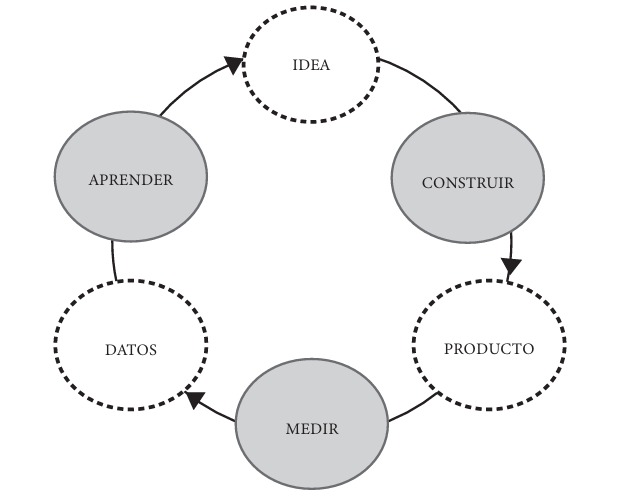
\includegraphics[width=0.7\textwidth]{Content/Images/cicloMetodologiaLean.jpeg}
        \footnote{Nota. \textup{Fuente: Lean Startup, creando productos escalables \cite{GioSyst3m}}}
\end{minipage}

Adoptando esta metodologia el proyecto se desarrollará de manera iterativa, permitiendo demostrar la viabilidad del producto y su aceptación en el mercado, minimizando riesgos y maximizando oportunidades de éxito. Además de permitir una rápida adaptación a los cambios del mercado y a las necesidades de los clientes, lo que es esencial para el éxito de un proyecto innovador como el propuesto.

La selección final del lugar se basará en un análisis detallado de los beneficios, costos y oportunidades que cada opción ofrece, con el objetivo de maximizar el impacto del proyecto tanto en línea como en el entorno local.

\subsection{Equipo de trabajo}
El equipo de trabajo esta compuesto por profesionales altamente capacitados y con capacidades transversales, aportando un gran apoyo al desarrollo del proyecto. El equipo se conforma por:
\begin{itemize}
    \item \textbf{Gerente General / CEO:} Lidera la estrategia global, gestión de recursos y expansión del proyecto, asegurando su posicionamiento como referente en seguridad para nómadas digitales.
    
    \item \textbf{Líder de Tecnología (CTO):} Dirige el desarrollo de la plataforma, enfocandose en la buena experiencia del usuario y la escalabilidad de la misma.
    
    \item \textbf{Director de Operaciones } Supervisa la red de recomendaciones , el algoritmo de evaluación de riesgos y las alianzas con entidades que presten servicios al publico deseado,Con la finalidad de evolucionar continuamente el proyecto basandose en los objetivos y estrategias planteadas.
\end{itemize}
\begin{adjustbox}{
            center,
            caption=[{Equipo de trabajo.}]{Equipo de trabajo. },
            label={EquipoDeTrabajo},
            nofloat=table, vspace={20px}}
            \resizebox{\textwidth}{!}{
            \begin{threeparttable}
            \begin{tabular}{|cllll|cllll|}
            \hline
            \multicolumn{5}{|c|}{\cellcolor[HTML]{D9EAD3}Integrante} & \multicolumn{5}{c|}{\cellcolor[HTML]{D9EAD3}Rol}                                          \\ \hline
            \multicolumn{5}{|c|}{Andrés Felipe Bejarano Barón}        & \multicolumn{5}{c|}{Gerente general, líder de la área de ingeniería}                      \\ \hline
            \multicolumn{5}{|c|}{Jeferson David Nieto Gaona}   & \multicolumn{5}{c|}{Directora del departamento de investigación, desarrollo e innovación} \\ \hline
            \end{tabular}%
            
            \begin{tablenotes}[para,flushleft]
                \vspace{2mm}
                \textit Nota. Fuente : Autores.
            \end{tablenotes}
            \end{threeparttable} 
            }    
    \end{adjustbox}
